\lab{Applications}{Beam Buckling}{Beam Buckling}

\objective{Use finite difference approximations and eigenvalues to approximate the strength of various types of beams.}

In many engineering applications it is desirable to be able to test how strong a structure will be prior to actually building it. In this lab we will explore the strength of a simple beam using mathematical techniques.

We can model a beam supporting a load $P$ by the following equation:

\[
EI \frac{d^2 y}{dx^2} = -P y
\]

\begin{figure}
\begin{center}
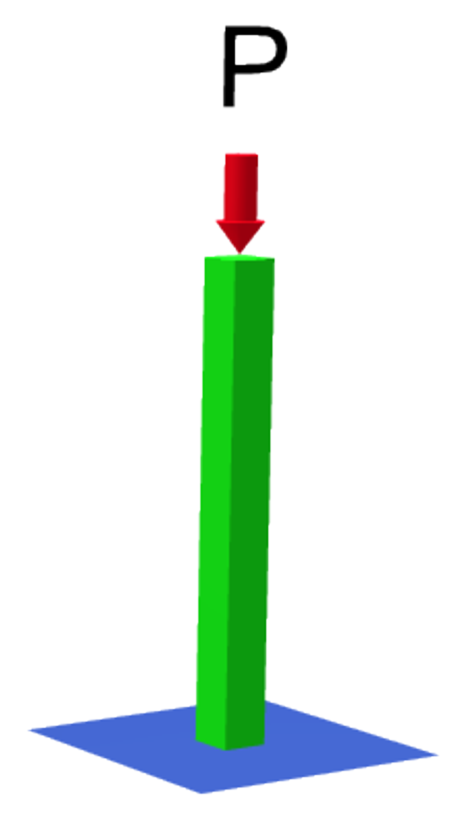
\includegraphics[scale = .3]{./Figures/Buckling.pdf}
\caption{A beam supporting a load $P$}
\label{Fig:Beam}
\end{center}
\end{figure}

This scenario is shown in figure \ref{Fig:Beam}. The variable $x$ is up and down, and $y$ is a lateral displacement (left or right). We have really simplified this problem to two dimensions, but the simplification is still representative in this case. We also have the boundary conditions that:

\[
y(0) = y(L) =0
\]

This specifies that the position of the top and bottom boundaries of the column are fixed (as would be the case in a building). In these equations $L$ is the length of the column, $E$ is known as the elastic modulus (representing the rigidity of the material) and $I$ represents the area moment of inertia (representing how the geometry resists deformation).

We can solve this equation using finite difference approximations. Recall that one approximation of the second derivative of a function is the following:

\[
y''(x_k) = \frac{y(x_k-1) - 2y(x_k) + y(x_{k+1}}{h^2}
\]

So, if we select the points

\[
x_k = \frac{kL}{n}
\]

For $k = 0\ldots n$ then we can rewrite our differential equation in the form:

\[
\frac{EIAy}{h^2} = -Py
\]

Where $y$ is a vector of length $n-1$ representing our function values at all of the $x_k$ (except for $k=0$ and $k=n$, which are determined by the boundary conditions), $h = \frac{L}{n}$ and $A$ is a matrix with $-2$ on the diagonal and $1$ on the super and sub-diagonal, as specified by the finite difference approximation above. Note that we incorporated our boundary conditions in the corners of the matrix (the derivative is only approximated by two terms there, since the third term in each case is the boundary term that is fixed at zero).

Clearly for any value of $P$ the equation has a trivial solution ($y=0$). However, by calculating the eigenvalues we can find the values of $P$ for which the equation has a non-trivial solution. Recall that any multiple of an eigenvector will still be an eigenvector. This means that when $P$ is an eigenvalue there are arbitrarily small non-trivial solutions to the differential equation. This tells us that the trivial solution is actually unstable whenever $P$ is an eigenvalue. Accordingly, the smallest eigenvalue of the system will be the value where the beam buckles and the system fails (in this system all of the eigenvalues turn out to have the correct sign, therefore giving physically meaningful values of $P$).

\begin{problem}
Find the load at which a five foot column of concrete with diameter of one foot will buckle. The modulus of elasticity for concrete is approximately $4.35$ million pounds per square inch. The area moment of inertia in this case is $I = \pi r^4/4$. The only necessary unit conversion is inches to feet (in the modulus of elasticity). The answer should be in $10^7$lbs (you only need to use vectors of moderate size to get an accurate answer: try n=100). What if instead the column is twenty feet long?
\end{problem}

One point of interest is related to the area moment of inertia. Given a fixed amount of material it actually turns out that the area moment of inertia is greater for a hollow tube than a solid column. This tells us that hollow tubes actually have a higher buckling strength than solid ones. In fact, I-beams are actually designed to increase area moment of inertia, which is why they are seen so often in construction.

It turns out we can actually solve this equation analytically. The non-trivial solutions to this type of equation are sines. We can thus deduce, using the chain rule that the eigenvalues of the derivative operator (neglecting the constants E and I) are
\[
\lambda_n = \frac{\pi^2 n^2}{L^2}
\]
for $n \in \mathbb{N}$. Thus we have that the buckling force is:
\[
F = \frac{\pi^2 EI}{L^2}
\]
Which, as you can verify, matches the solution found above very nicely.

So if we can solve this solution analytically why do we bother with the finite difference approximation? Suppose instead that our column is made of two types of concrete, the bottom half with $E = 4.35\times 10^6$ and the other half with$E = 1 \times 10^6$. This type of problem is more difficult to solve analytically. However, if we modify our finite difference equation to compensate for the differences in the material we can still solve the problem. We can re-write the equation:

\[
B A y = -Py
\]
Where B is a matrix with the value of $E I$ at each $x_k$ on the diagonal. So in our example above B would be the following matrix:

\begin{matlab}
\begin{lstlisting}[style=matlab]
B = r^4/4 *diag([4.35*ones(1,50) ones(1,50)])*1e6
\end{lstlisting}
\end{matlab}

\begin{problem}
Suppose that the bottom third of our column is made of aluminum ($E = 10^7$), the middle third is concrete and the top third is made of nylon ($E = 5\times 10^5$). What is the buckling strength of the column? If the order of the materials is changed does this affect the buckling strength?
\end{problem}



